\documentclass[11pt]{beamer}

\usetheme{Madrid}
%\usepackage{palatino} % ← Commenté temporairement

\setbeamertemplate{footline}{
  \leavevmode%
  \hbox{%
    \begin{beamercolorbox}[wd=0.4\paperwidth,ht=2.5ex,dp=1ex,left]{author in head/foot}%
      \usebeamerfont{author in head/foot}\hspace{1em}\insertshortauthor
    \end{beamercolorbox}%
    \begin{beamercolorbox}[wd=0.30\paperwidth,ht=2.5ex,dp=1ex,center]{title in head/foot}%
      \usebeamerfont{title in head/foot}\insertshorttitle
    \end{beamercolorbox}%
    \begin{beamercolorbox}[wd=0.3\paperwidth,ht=2.5ex,dp=1ex,right]{date in head/foot}%
      \usebeamerfont{date in head/foot}\insertshortdate{} \hspace{1em}
      \insertframenumber{} / \inserttotalframenumber\hspace{1em}
    \end{beamercolorbox}%
  }%
  \vskip0pt%
}

\usepackage{listings}
\usepackage{xcolor}

\lstdefinestyle{sqlStyle}{
  language=SQL,
  basicstyle=\ttfamily\small,
  keywordstyle=\color{blue},
  stringstyle=\color{teal},
  commentstyle=\color{gray},
  morekeywords={SUM, USING, JOIN, GROUP, ORDER, BY},
  breaklines=true,
  captionpos=b
}

\setbeamertemplate{navigation symbols}{}
\setbeamercovered{transparent}

\title[Présentation]{Avancement SAE}
\subtitle{S2.01 Conception et implémentation d'une base de données}

\author[Ibrahim BENKHERFELLAH \and Axel COULET]{Ibrahim BENKHERFELLAH \and Axel COULET}
\institute[USPN]{Université Sorbonne Paris Nord \\BUT1 SD \- Semestre 2}
\date[\today]{\today}

\begin{document}

\maketitle

\begin{frame}
  \frametitle{Table des matières}
  \tableofcontents
\end{frame}

\section{Introduction}
\begin{frame}
  \frametitle{Objectif du projet}
  \begin{itemize}
    \item<1-> Comprendre et modéliser le commerce des technologies à faible émission de carbone.
    \item<2-> Concevoir une base de données normalisée à partir de deux jeux de données CSV.
    \item<3-> Interroger et visualiser les données pour produire des analyses pertinentes.
  \end{itemize}
\end{frame}

\section{Exploration et compréhension des données}
\begin{frame}
  \frametitle{Étude des sources de données}
  \begin{itemize}
    \item Fichiers CSV étudiés :
      \begin{itemize}
        \item<1-> \texttt{\href{https://climatedata.imf.org/datasets/1d33174e9e46429d9e570d539556f66a/explore}{Trade\_in\_Low\_Carbon\_Technology\_Products.csv}}
        \item \texttt{\href{https://climatedata.imf.org/datasets/975bc577fe7342c2a3651e8841959c47_0/explore}{Bilateral\_Trade\_in\_Low\_Carbon\_Technology\_Products.csv}}
      \end{itemize}
    \item<2-> Exploration initiale avec Python (pandas) : \\
          \texttt{.head()}, \texttt{.info()}, etc.
    \item<3-> Identification de colonnes clés : \texttt{CTS\_Code}, \texttt{Indicator}, \texttt{Trade\_Flow}, etc.
    \item<4-> Difficultés rencontrées :
    	\begin{itemize}
    	\item Colonnes de dates (comme Year) au mauvais format ou non reconnues comme Date.
    	\item Colonnes "F1994" à "F2023" en format long à dépivoter (via \text{UNPIVOT} de SQL).
    	\end{itemize}
  \end{itemize}
\end{frame}

\begin{frame}
  \frametitle{Sources et structuration des fichiers}
  \begin{itemize}
    \item<1-> Données structurées en colonnes d'années : F1994 à F2023.
    \item<2-> Présence de colonnes de description redondantes (\texttt{CTS\_Code}, \texttt{CTS\_Name}, \texttt{CTS\_Full\_Descriptor}).
    \item<3-> Première étape : lecture manuelle pour repérage des redondances et structures tabulaires.
  \end{itemize}
\end{frame}

\begin{frame}
  \frametitle{Préparation et normalisation des données}
  \begin{itemize}
    \item<1-> Conversion des colonnes FXXXX en format court (année, valeur).
    \item<2-> \text{Normalisation des années (F1994 à F2023)} :
    \begin{itemize}
      \item Chaque colonne FXXXX devient une ligne avec une valeur d'année.
      \item Transformation effectuée via \texttt{UNION ALL} dans SQL pour correspondre à la logique de \texttt{stack()} en Python.
    \end{itemize}
    \item<3-> Problèmes rencontrés :
    \begin{itemize}
      \item Ambiguïté sur le pays origine.
      \item Duplication de lignes si filtrage incorrect.
    \end{itemize}
  \end{itemize}
\end{frame}

\begin{frame}
  \frametitle{Transformation des données : format large vers format long}

  \textbf{Format large (wide)} :\newline
  Chaque année est une colonne
  
  \begin{tabular}{|c|c|c|c|c|}
    \hline
    ... & Scale & F1994 & F1995 & F1996 \\
    \hline
    ... & Units & 190885.0 & 2433262.0 & 17679060.0 \\
    ... & Units & 0.0004146 & 0.0053298 & 0.0347023 \\
    ... & Units & 668268200.0 & 612865500.0 & 493126000.0 \\
    \hline
  \end{tabular}

  \vspace{1em}
  \centering
  $\Downarrow$
  \vspace{1em}

  \raggedright
  \textbf{Format long (tidy)} :\newline
  Chaque ligne correspond à une observation unique (année, valeur).

  \begin{tabular}{|c|c|c|c|}
    \hline
    ... & Scale & Year & Value \\
    \hline
    ... & Units & F1994 & 190885.0 \\
    ... & Units & F1994 & 0.0004146 \\
    ... & Units & F1994 & 668268200.0 \\
    \hline
  \end{tabular}

\end{frame}



\begin{frame}
  \frametitle{Données structurées et décisions clés}
  \begin{itemize}
    \item<1-> Création d'une table \texttt{Bilateral\_Trade} pour les données bilatérales :
    \begin{itemize}
      \item Relation réflexive entre deux pays (deux clés étrangères vers \texttt{country}).
    \end{itemize}
    \item<2-> Table \texttt{Trade} pour les données nationales.
    \item<3-> Lien systématique aux dimensions : pays, indicateur, catégorie, année.
  \end{itemize}
\end{frame}

\section{Modélisation de la base de données}

\begin{frame}
	\frametitle{Schéma Entité-Association}
	
	\begin{figure}
		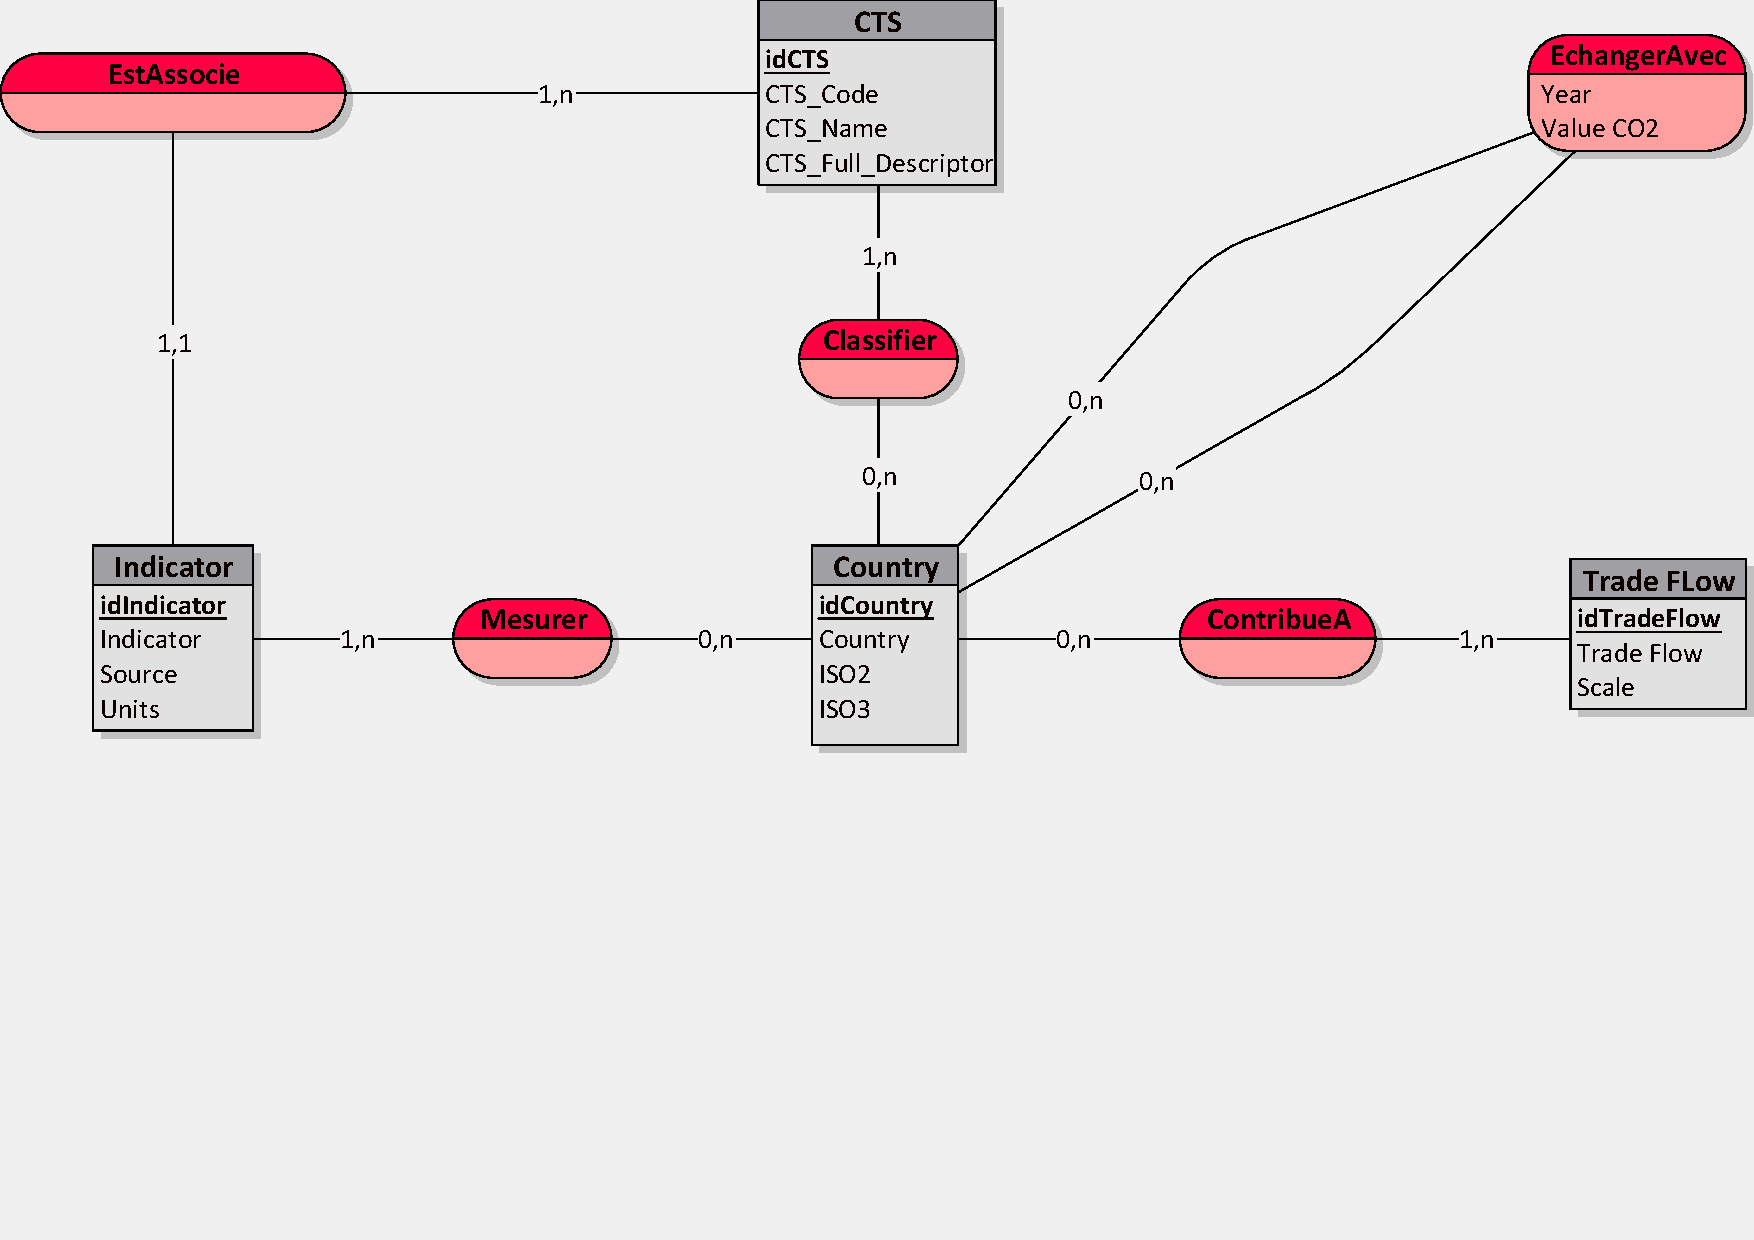
\includegraphics[width=0.8\linewidth]{../schema_ea/schema_EA_initial.pdf}
		\caption{Schéma Entité-Association Initial}
	\end{figure}
\end{frame}


\begin{frame}
	\frametitle{Schéma Entité-Association}
	
	\begin{figure}
		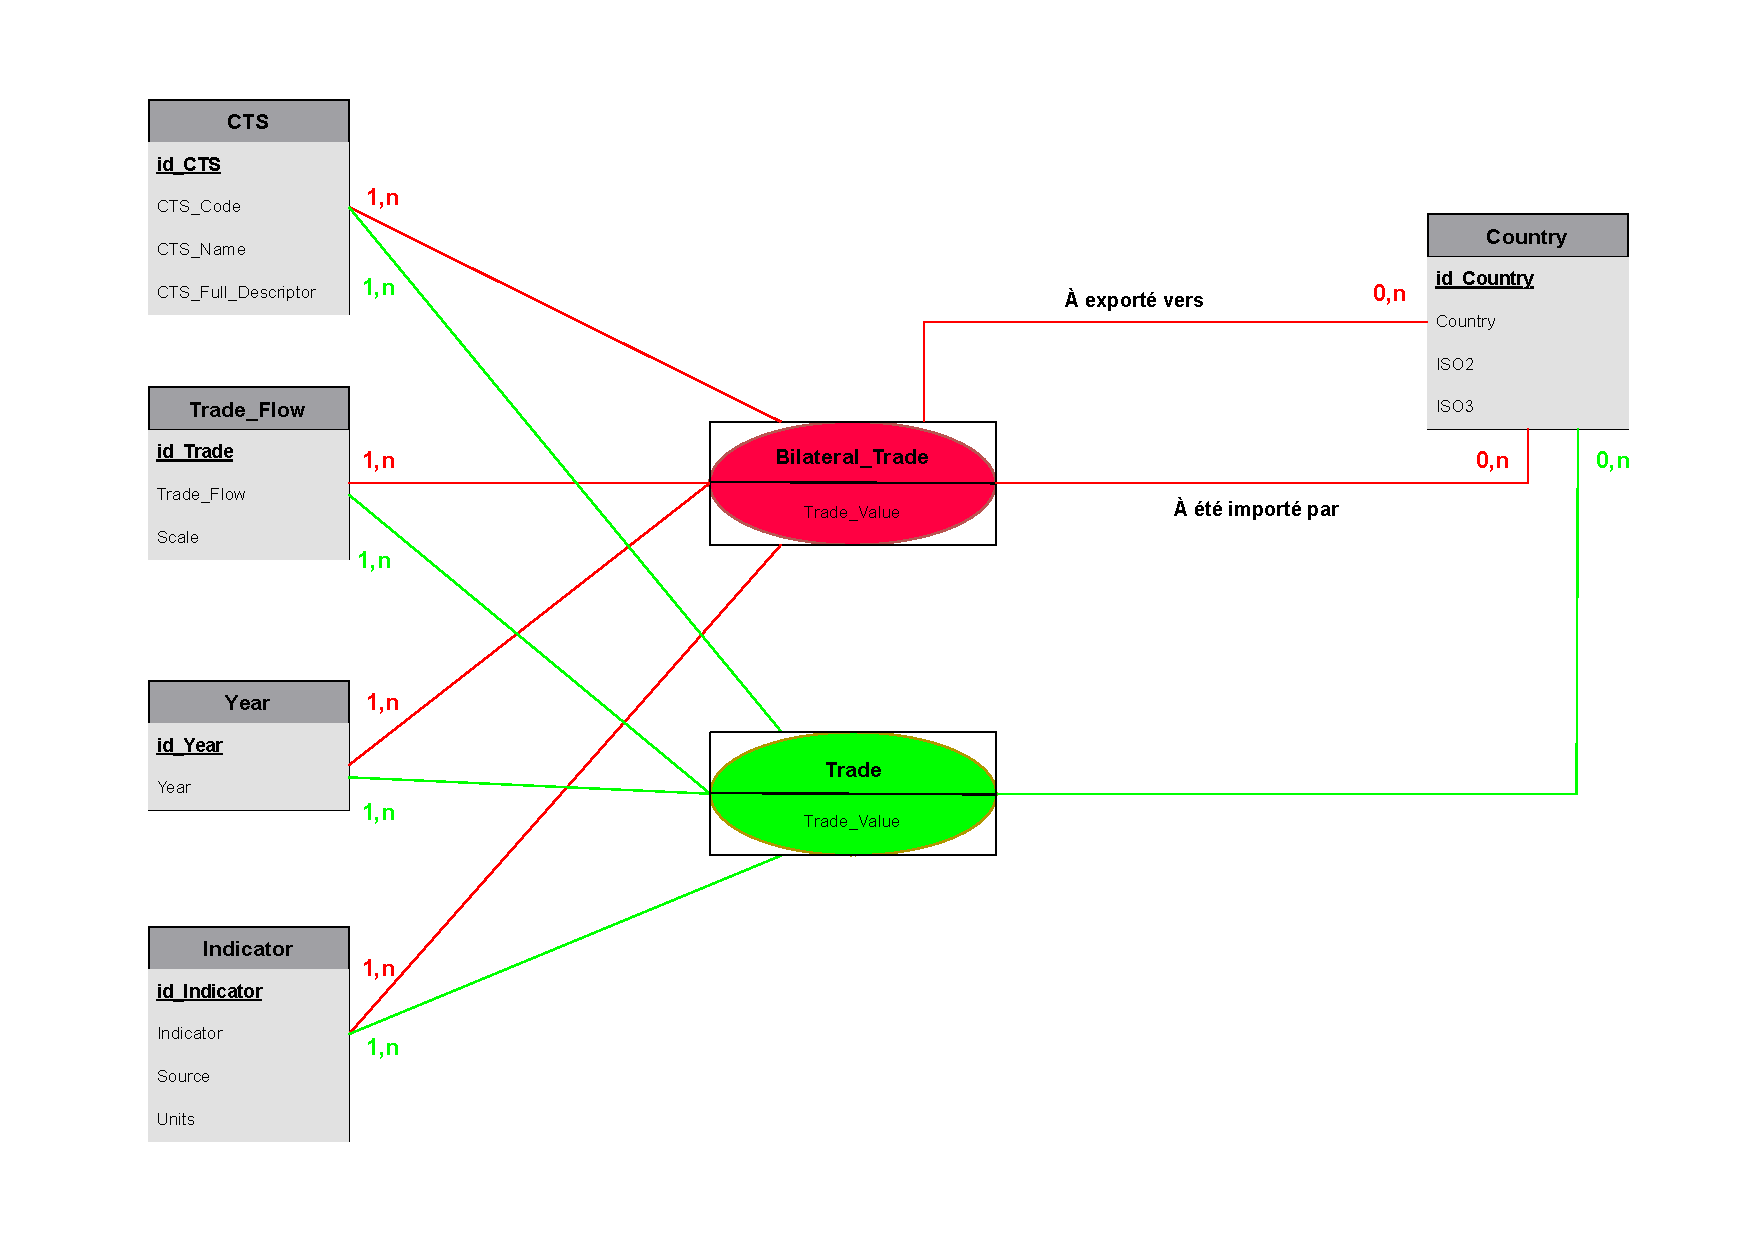
\includegraphics[width=0.8\linewidth]{../schema_ea/schema_EA_final.pdf}
		\caption{Schéma Entité-Association Final}
	\end{figure}
\end{frame}


\begin{frame}
  \frametitle{Modèle conceptuel (EA)}
  \begin{itemize}
    \item<1-> Type Entités : \texttt{Country}, \texttt{Indicator}, \texttt{CTS}, \texttt{Trade\_Flow}, \texttt{Year}
    \item<2-> Type Associations : 
      \begin{itemize}
        \item \texttt{Bilateral\_Trade} (réflexive sur \texttt{Country})
        \item \texttt{Trade} (relation simple avec agrégation)
      \end{itemize}
    \item<3-> Justification des cardinalités et des relations
  \end{itemize}
\end{frame}

\begin{frame}
  \frametitle{Structure relationnelle finale}
  \begin{itemize}
    \item Schéma relationnel résultant de la modélisation EA :
    \begin{itemize}
      \item \texttt{Country(\underline{idCountry}, Country, ISO2, ISO3)}
      \item \texttt{CTS(\underline{idCTS}, CTS\_Code, CTS\_Name, CTS\_Full\_Descriptor)}
      \item \texttt{Trade\_Flow(\underline{id\_Trade\_Flow}, Trade\_Flow, Scale)}
      \item \texttt{Indicator(\underline{idIndicator}, Indicator, Source, Units)}
      \item \texttt{Year(\underline{id\_Year}, Year)}
      \item \texttt{Bilateral\_Trade(\underline{id\_country}, \underline{id\_counterpart}, \underline{id\_indicator}, \underline{id\_cts}, \underline{id\_Trade\_Flaw}, \underline{id\_year}, trade\_value)}
      \item \texttt{Trade(\underline{id\_country}, \underline{id\_indicator}, \underline{id\_cts}, \underline{id\_Trade\_Flaw}, \underline{id\_year}, trade\_value)}
    \end{itemize}
  \end{itemize}
\end{frame}

\begin{frame}
  \frametitle{Forme normale : 1NF}
  \begin{itemize}
    \item Toutes les valeurs sont atomiques : aucun champ multivalué ou composé.
    \item Transformation des colonnes F1994 à F2023 en une colonne \texttt{id\_year} via pivot SQL.
    \item Tables relationnelles sans redondance horizontale.
    \item \textbf{Conclusion} : le schéma respecte la \textbf{première forme normale (1NF)}.
  \end{itemize}
\end{frame}

\begin{frame}
  \frametitle{Forme normale : 2NF}
  \begin{itemize}
    \item Le schéma est en 1NF.
    \item Aucune dépendance fonctionnelle partielle dans les tables à clés composites.
    \item Exemple : les descripteurs CTS ont été extraits dans une table distincte, reliée par \texttt{CTS\_Code}.
    \item \textbf{Conclusion} : toutes les dépendances fonctionnelles concernent la clé entière → \textbf{2NF validée}.
  \end{itemize}
\end{frame}

\begin{frame}
  \frametitle{Forme normale : 3NF}
  \begin{itemize}
    \item Le schéma est en 2NF.
    \item Suppression des dépendances transitives.
    \item Exemple : l’unité d’un indicateur dépend uniquement de l’indicateur, pas d’un pays ou autre entité.
    \item \textbf{Conclusion} : toutes les colonnes non-clés dépendent uniquement de la clé primaire → \textbf{schéma en 3NF}.
  \end{itemize}
\end{frame}

\begin{frame}
  \frametitle{Forme normale : BCNF}
  \begin{itemize}
    \item Toutes les dépendances fonctionnelles ont un antécédent qui est une super-clé.
    \item Exemple : dans \texttt{Bilateral\_Trade}, seule la combinaison complète des identifiants détermine \texttt{trade\_value}.
    \item Il n'existe pas de dépendance fonctionnelle violant cette condition.
    \item \textbf{Conclusion} : le schéma respecte la forme normale de \textbf{Boyce-Codd (BCNF)}.
  \end{itemize}
\end{frame}


\section{Script de création et peuplement SQL}
\begin{frame}[fragile]
  \frametitle{Création de la table \texttt{Country}}
\begin{verbatim}
CREATE TABLE Country(
   id_Country SMALLSERIAL PRIMARY KEY,
   Country VARCHAR(50),
   ISO2 CHAR(2),
   ISO3 CHAR(3)
);
\end{verbatim}
\end{frame}

\begin{frame}[fragile]
  \frametitle{Création de la table \texttt{Indicator}}
\begin{verbatim}
CREATE TABLE Indicator(
   id_Indicator SMALLSERIAL PRIMARY KEY,
   Indicator VARCHAR(80),
   Source VARCHAR,
   Units VARCHAR(50),
   Scale VARCHAR(5)
);
\end{verbatim}
\end{frame}

\begin{frame}[fragile]
  \frametitle{Création de la table \texttt{CTS}}
\begin{verbatim}
CREATE TABLE CTS(
   id_CTS SMALLSERIAL PRIMARY KEY,
   CTS_Code VARCHAR(6),
   CTS_Name VARCHAR(100),
   CTS_Full_Descriptor VARCHAR(150)
);
\end{verbatim}
\end{frame}

\begin{frame}[fragile]
  \frametitle{Création de la table \texttt{Trade\_Flow}}
\begin{verbatim}
CREATE TABLE Trade_Flow(
   id_Trade_Flow SMALLSERIAL PRIMARY KEY,
   Trade_Flow VARCHAR(20)
);
\end{verbatim}
\end{frame}

\begin{frame}[fragile]
  \frametitle{Création de la table \texttt{Year}}
\begin{verbatim}
CREATE TABLE Year(
   id_Year SMALLSERIAL PRIMARY KEY,
   Year DATE
);
\end{verbatim}
\end{frame}

\begin{frame}[fragile]
  \frametitle{Création de la table \texttt{Bilateral\_Trade}}
\begin{verbatim}
CREATE TABLE Bilateral_Trade (
    id_Country SMALLINT REFERENCES Country(id_Country),
    id_Counterpart SMALLINT REFERENCES Country(id_Country),
    id_Indicator SMALLINT REFERENCES Indicator(id_Indicator),
    id_CTS SMALLINT REFERENCES CTS(id_CTS),
    id_Trade_Flow SMALLINT REFERENCES Trade_Flow(...),
    id_Year SMALLINT REFERENCES Year(id_Year),
    trade_value DOUBLE PRECISION,
    PRIMARY KEY(id_Country, id_Counterpart_Country,
                id_Indicator, id_CTS, id_Trade_Flaw, id_Year)
);
\end{verbatim}
\end{frame}

\begin{frame}[fragile]
  \frametitle{Création de la table \texttt{Trade}}
\begin{verbatim}
CREATE TABLE Trade (
    id_Country SMALLINT REFERENCES Country(id_Country),
    id_Indicator SMALLINT REFERENCES Indicator(id_Indicator),
    id_CTS SMALLINT REFERENCES CTS(id_CTS),
    id_Trade_Flow SMALLINT REFERENCES Trade_Flow(...),
    id_Year SMALLINT REFERENCES Year(id_Year),
    trade_value DOUBLE PRECISION,
    PRIMARY KEY(id_Country, id_Indicator, id_CTS, 
    id_Trade_Flaw, id_Year)
);
\end{verbatim}
\end{frame}


\begin{frame}
  \frametitle{Peuplement de la base}
  \begin{itemize}
    \item<1-> Utilisation de \texttt{COPY}, \texttt{INSERT INTO} avec jointures.
    \item<1-> Alignement avec les traitements Python (\texttt{Avec .stack()}).
    \item<1-> Cas particuliers traités : 
      \begin{itemize}
        \item Échanges d’un pays avec lui-même
        \item Lignes \texttt{NULL} / Trade Flow = Not Applicable
      \end{itemize}
    \item<2-> Difficultés rencontrées :
    	\begin{itemize}
  			\item Contraintes techniques : \texttt{NULL}, unicité, jointures complexes.
  			\item Problèmes de données : fusion sans doublons, nettoyage, volume élevé.
		\end{itemize}
    \end{itemize}
\end{frame}

\section{Interrogation et visualisation des données}
\begin{frame}
  \frametitle{Requêtes d’analyse}
  \begin{itemize}
    \item Top 10 des pays importateurs de technologies en provenance de Chine (2021)
    \item Répartition mondiale des exportations de technologies en 2021 (\%)
    \item Part annuelle des échanges bilatéraux vs nationaux dans le commerce mondial (1994 à 2023)
    \item Nombre de pays importateurs depuis la Chine (2021)
    \item Nombre de flux d’exportation de la Chine enregistrés (2021)
    \item Valeur totale des exportations de la Chine (2021)
  \end{itemize}
\end{frame}

\begin{frame}
  \frametitle{Visualisation}
  \begin{itemize}
    \item Utilisation de Metabase pour interroger la BD
    \item Utilisation de Tableau pour valider les valeurs issues du CSV
    \item Comparaison SQL / Python → vérification de l’intégrité
    \item Exemples visuels :
  \end{itemize}
\end{frame}


\begin{frame}[fragile]
  \frametitle{Tableau de Bord - Étude sur la Chine}
  \begin{figure}
    \centering
    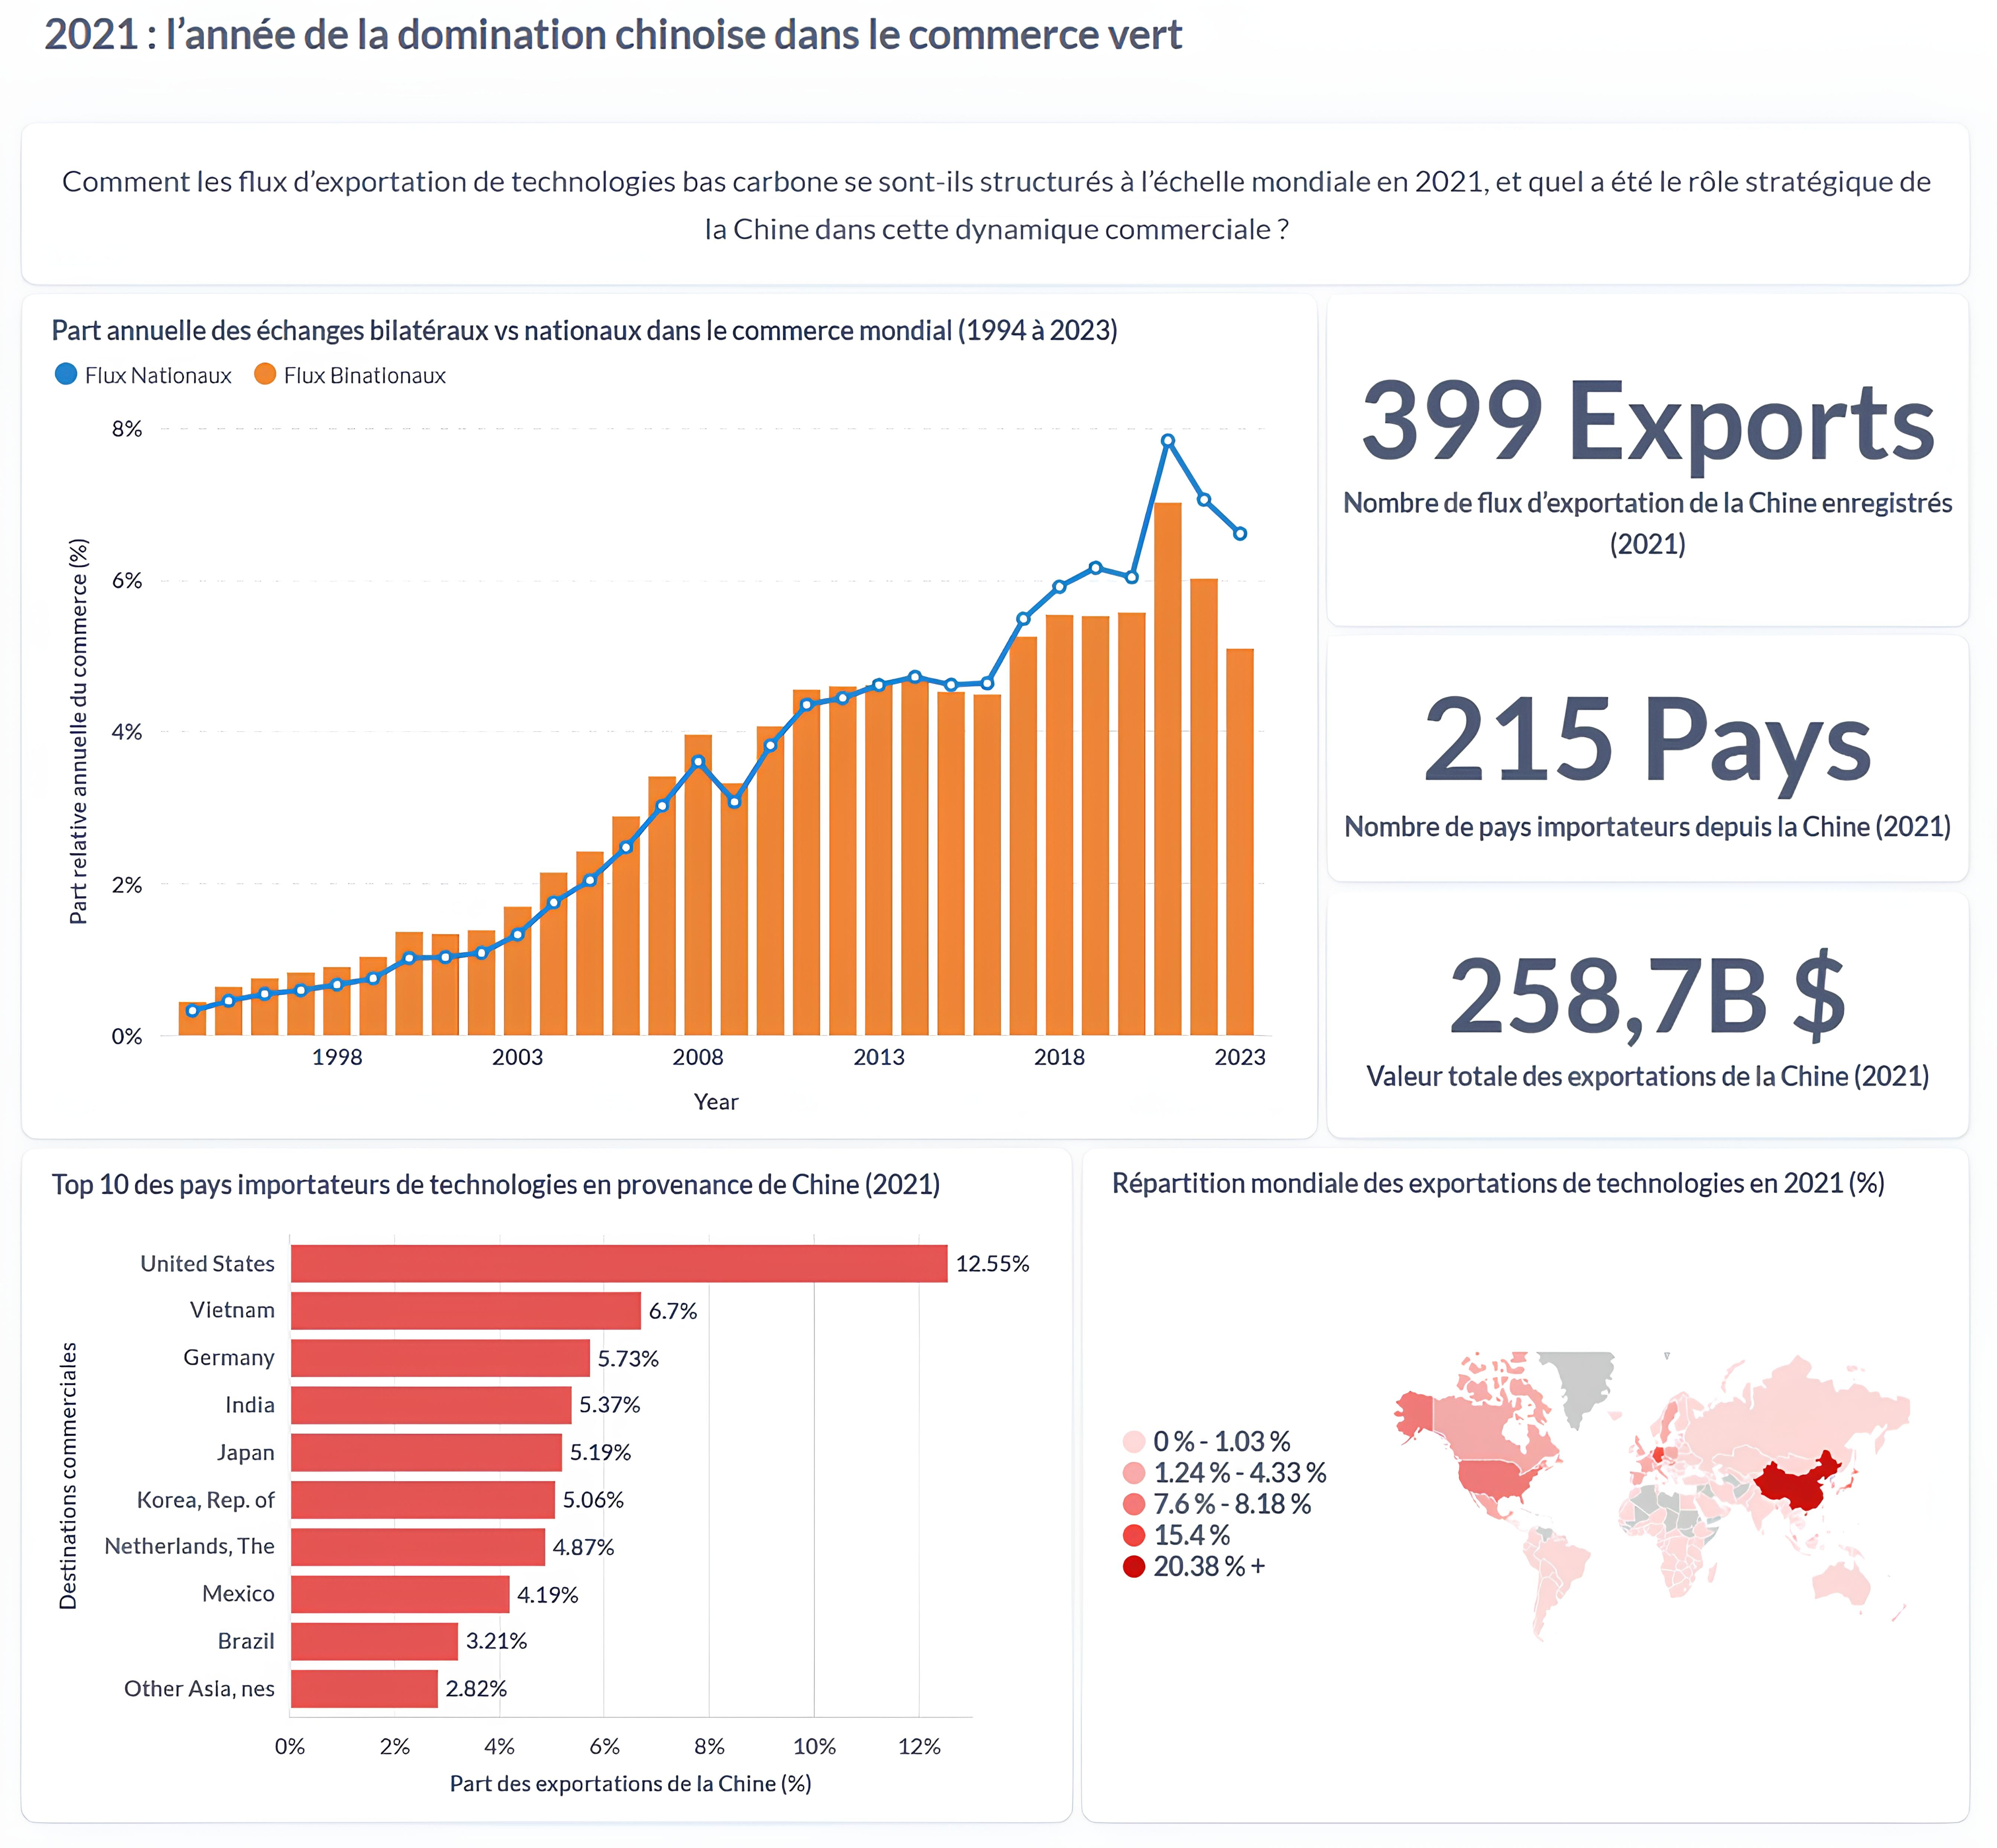
\includegraphics[width=0.625\linewidth]{../script_dataviz/dash-board}
    \caption{2021 : L'année de la domination chinoise dans le commerce vert}
  \end{figure}
\end{frame}

\section{Conclusion}
\begin{frame}
  \frametitle{Bilan du projet}
  \begin{itemize}
    \item Base de données fonctionnelle et fidèle au CSV (dans nos rêves)
    \item Respect des étapes du processus de modélisation
    \item Difficultés sur l’import (pivot, valeurs nulles, sens du flux)
    \item Vérification croisée avec Python
    \item Améliorations possibles :
  \end{itemize}
\end{frame}

\begin{frame}
  \frametitle{Merci pour votre attention}
  \begin{center}
    \huge \textbf{Questions ?}
  \end{center}
\end{frame}

\end{document}